\documentclass[fleqn, a4paper, 11pt, oneside]{amsart}
%\usepackage[top = 2cm, bottom = 1cm, left = 1cm, right = 1cm]{geometry}
\usepackage{exsheets, tasks}
\usepackage{amsmath, amssymb, amsthm} %standard AMS packages
\usepackage{marginnote} %marginnotes
\usepackage{gensymb} %miscellaneous symbols
\usepackage{commath} %differential symbols
\usepackage{xcolor} %colours
\usepackage{cancel} %cancelling terms
\usepackage[free-standing-units, space-before-unit]{siunitx} %formatting units
	\sisetup
	{
		per-mode=fraction,
		fraction-function=\frac
	}
\usepackage{tikz, pgfplots} %diagrams
\usetikzlibrary{calc, hobby, patterns, intersections, decorations.markings}
\usepackage{graphicx} %inserting graphics
\usepackage{hyperref} %hyperlinks
\usepackage{datetime} %date and time
\usepackage{ulem} %underline for \emph{}
\usepackage{xfrac} %inline fractions
\usepackage{enumerate,enumitem} %numbered lists
\usepackage{float} %inserting floats
\usepackage{circuitikz}[american voltages, american currents] %circuit diagrams
\usepackage[utf8]{inputenc}
\usepackage{booktabs}
\usepackage{todonotes}

\newcommand\numberthis{\addtocounter{equation}{1}\tag{\theequation}} %adds numbers to specific equations in non-numbered list of equations

\newcommand{\AxisRotator}[1][rotate=0]{
	\tikz [x=0.25cm,y=0.60cm,line width=.2ex,-stealth,#1] \draw (0,0) arc (-150:150:1 and 1);%
} %rotation symbols on axes

\theoremstyle{definition}
\newtheorem{example}{Example}
\newtheorem{definition}{Definition}

\theoremstyle{theorem}
\newtheorem{theorem}{Theorem}

\newcommand{\curl}{\mathrm{curl\,}}

\makeatletter
\@addtoreset{section}{part} %resets section numbers in new part
\makeatother

\renewcommand{\thesubsection}{(\arabic{subsection})}
\renewcommand{\thesection}{(\arabic{section})}

\renewcommand{\emph}{\uline}

\renewcommand{\tilde}{\widetilde}

%section headings on left
\makeatletter
\def\specialsection{\@startsection{section}{1}%
	\z@{\linespacing\@plus\linespacing}{.5\linespacing}%
	%  {\normalfont\centering}}% DELETED
	{\normalfont}}% NEW
\def\section{\@startsection{section}{1}%
	\z@{.7\linespacing\@plus\linespacing}{.5\linespacing}%
	%  {\normalfont\scshape\centering}}% DELETED
	{\normalfont\scshape}}% NEW
\makeatother

%forces newline after subsection
\makeatletter
\def\subsection{\@startsection{subsection}{3}%
	\z@{.5\linespacing\@plus.7\linespacing}{.1\linespacing}%
	{\normalfont\itshape}}
\makeatother

\settasks{counter-format = tsk[1].}

\SetupExSheets{solution/print = true}

%opening
\title{Quantum and Solid State Physics : Assignment 9}
\author
{
	Aakash Jog\\
	ID : 989323563
}
\date{\formatdate{24}{12}{2015}}

\begin{document}

\tikzset{->-/.style={decoration={
  markings,
  mark=at position #1 with {\arrow{>}}},postaction={decorate}}}

\maketitle
%\setlength{\mathindent}{0pt}

\begin{question}
	An N-type silicon sample with the following properties at room temperature is illuminated for a long time under low level injection conditions.
	\begin{align*}
		N_d    & = 10^{16} \si{\per\centi\metre\cubed} \\
		\tau_n & = 1 \si{\micro\second}                \\
		\tau_p & = 1 \si{\micro\second}
	\end{align*}
	At steady state, the excess carrier concentration is $\hat{n} = \hat{p} = 10^7 \si{\per\centi\metre\cubed}$.
	Illumination is stopped at $t = 0$.
	\begin{enumerate}
		\item
			What are the electron and hole concentrations $n$ and $p$ for $t < 0$?
		\item
			Write an expression for the hole concentration, $p(t)$, as a function of time for $t > 0$, and plot your result.
		\item
			At time $t = 1 \si{\milli\second}$, the sample is again illuminated, with the same conditions as for $t < 0$.
			What is the concentration of holes at $t = 1.001 \si{\milli\second}$?
	\end{enumerate}
\end{question}

\begin{solution}
	\begin{enumerate}[leftmargin=*]
		\item
			\begin{align*}
				n & = n_0 + \hat{n}  \\
                                  & = N_d + \hat{n}  \\
                                  & = 10^{16} + 10^7 \\
                                  & \approx 10^{16} \si{\per\centi\metre\cubed}
			\end{align*}
			\begin{align*}
				p & = p_0 + \hat{p}                                            \\
                                  & = \frac{{n_i}^2}{N_d} + \hat{p}                            \\
                                  & = \frac{\left( 1.5 \times 10^{10} \right)}{10^{16}} + 10^7 \\
                                  & = 2.25 \times 10^4 + 10^7                                  \\
                                  & \approx 10^7
			\end{align*}
		\item
			\begin{align*}
				\hat{p}(t) & = 10^7 e^{-\frac{t}{\tau_p}}  \\
                                           & = 10^7 e^{-\frac{t}{10^{-6}}} \\
                                           & = 10^7 e^{-10^6 t} \si{\per\centi\metre\cubed}
			\end{align*}
			Therefore,
			\begin{align*}
				p & = p_0 + \hat{p} \\
                                  & = 10^4 + 10^7 e^{-10^6 t}
			\end{align*}
			Therefore,
			\begin{figure}[H]
				\centering
				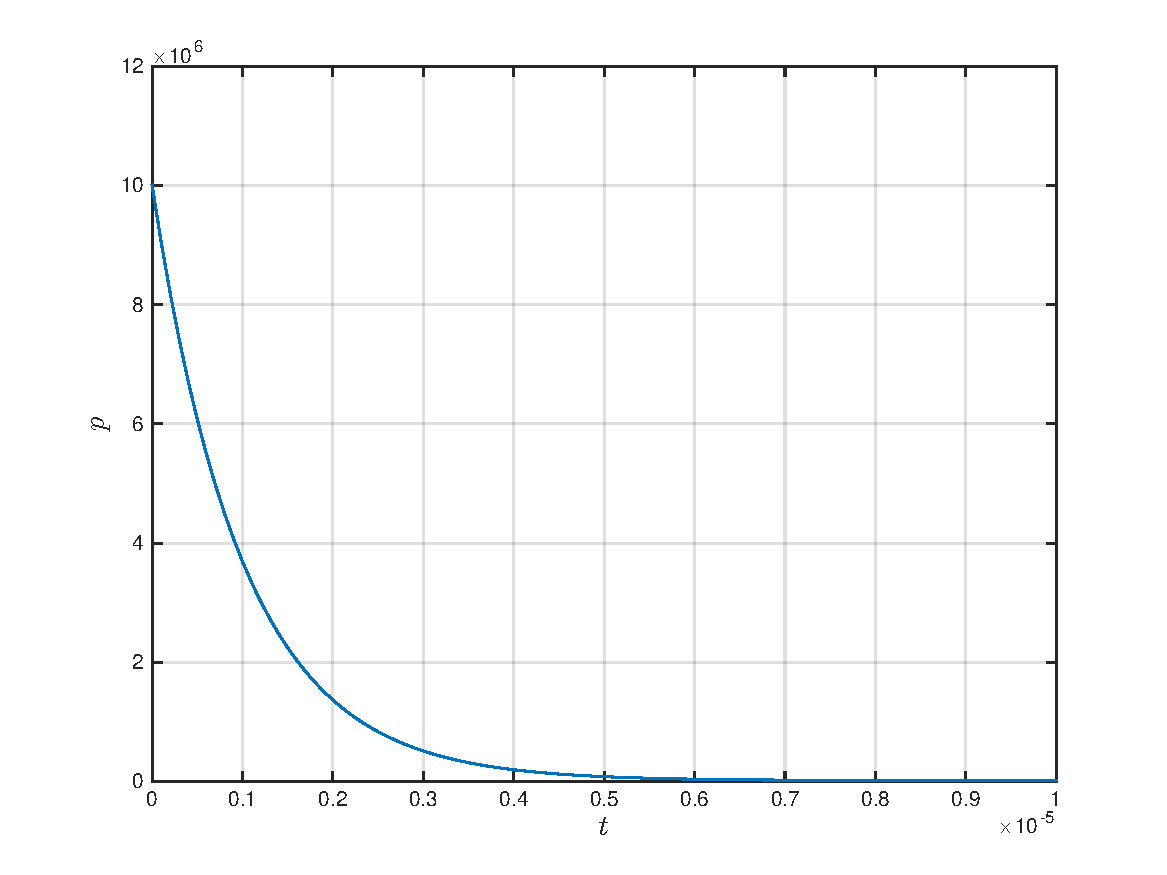
\includegraphics[width = 0.8\textwidth]{plot1.pdf}
			\end{figure}
		\item
			\begin{align*}
				\hat{p}(t_0 = 10^{-3} \si{\second}) & = 10^7 e^{-10^6 \cdot 10^{-3}} \\
                                                                    & = 10^7 e^{-10^3}               \\
                                                                    & \approx 0
			\end{align*}
			Therefore,
			\begin{align*}
				\hat{p}(t) & = \left( 1 - \frac{1}{e} \right) \hat{p}(0) \\
                                           & = \frac{e - 1}{e} 10^7                      \\
                                           & \approx 6.3 \times 10^6 \si{\per\centi\metre\cubed}
			\end{align*}
			Therefore,
			\begin{align*}
				p & = p_0 + \hat{p}          \\
                                  & = 10^4 + 6.4 \times 10^6 \\
                                  & \approx 6.3 \times 10^6 \si{\per\centi\metre\cubed}
			\end{align*}
	\end{enumerate}
\end{solution}

\begin{question}
	A P-type silicon sample, with the following properties, doping $N_a$, minority carrier lifetime $\tau_n$, at room temperature is illuminated uniformly throughout the volume of the sample, for a long time, with an optical generation rate of $G_{\text{optical}} \si{\per\centi\metre\cubed\per\second}$.
	Then, at time $t = 0$, the light intensity is reduced, and for $t > 0$, the optical regeneration rate is half of the value as before, i.e.,
	\begin{align*}
		G_{\text{optical}}(t > 0) & = \frac{1}{2} G_{\text{optical}}(t < 0)
	\end{align*}
	Assume low level injection over all time.
	Determine the equation for excess electron carrier concentration, $\hat{n}(t)$, as a function of time, for $t > 0$.
\end{question}

\begin{solution}
	For $t > 0$,
	\begin{align*}
		\dod{\hat{n}}{t} & = \frac{G_{\text{optical}}}{2} - \frac{\hat{n}}{\tau_n}
	\end{align*}
	For $t = 0$,
	\begin{align*}
		\hat{n} & = G_{\text{optical}} \tau_n
	\end{align*}
	Therefore, solving the ODE,
	\begin{align*}
		\hat{n} & = \frac{G_{\text{optical}} \tau_n}{2} \left( 1 + e^{-\frac{t}{\tau_n}} \right)
	\end{align*}
\end{solution}

\begin{question}
	Consider the following potential.
	\begin{align*}
		V(x) &=
			\begin{cases}
				0   & ;\quad x < 0 \\
				V_0 & ;\quad x > 0 \\
			\end{cases}
	\end{align*}
	A particle with mass $m$ is approaching the potential from the left.
	The energy of the particle can be either $0 < E < V_0$, or $E > V_0$.
	\begin{enumerate}
		\item Write the general solution to the time independent Schrödinger equation for a particle with $E > V_0$.
		\item Write the general solution to the time independent Schrödinger equation for a particle with $ 0 < E < V_0$.
		\item Write down the boundary conditions required to find the constants from the above parts.
		\item Write an expression for the transmission and reflection coefficients for the case $E > V_0$.
		\item Write an expression for the transmission and reflection coefficients for the case $0 < E < V_0$.
	\end{enumerate}
\end{question}

\begin{solution}
	\begin{enumerate}[leftmargin=*]
		\item
			Let
			\begin{align*}
				k_1 & = \sqrt{\frac{2 m E}{\hbar^2}} \\
				k_2 & = \sqrt{\frac{2 m (E - V_0)}{\hbar^2}}
			\end{align*}
			For $E > V_0$,
			\begin{align*}
				\psi(x) &=
					\begin{cases}
						A_1 e^{i k_1 x} + B_1 e^{-i k_1 x} & ;\quad x < 0 \\
						C_1 e^{i k_2 x}                    & ;\quad x > 0 \\
					\end{cases}
			\end{align*}
		\item
			Let
			\begin{align*}
				k_3 & = \sqrt{\frac{2 m E}{\hbar^2}} \\
				k_4 & = \sqrt{\frac{-2 m (E - V_0)}{\hbar^2}}
			\end{align*}
			For $0 < E < V_0$,
			\begin{align*}
				\psi(x) &=
					\begin{cases}
						A_2 e^{i k_3 x} + B_2 e^{-i k_3 x} & ;\quad x < 0 \\
						C_2 e^{-k_4 x}                     & ;\quad x > 0 \\
					\end{cases}
			\end{align*}
		\item
			As the jump at $x = 0$ is finite, $\psi$ and $\psi'$ must be continuous at $x = 0$.\\
			Therefore, for $E > V_0$,
			\begin{align*}
				A_1 + B_1       & = C_1 \\
				(A_1 - B_1) k_1 & = C_1 k_2
			\end{align*}
			Therefore, solving,
			\begin{align*}
				\frac{B_1}{A_1} & = \frac{k_1 - k_2}{k_1 + k_2} \\
				\frac{C_1}{A_1} & = \frac{2 k_1}{k_1 + k_2}
			\end{align*}
			Therefore, for $0 < E < V_0$,
			\begin{align*}
				A_2 + B_2       & = C_2 \\
				(A_2 - B_2) k_3 & = i C_2 k_4
			\end{align*}
			Therefore, solving,
			\begin{align*}
				\frac{B_2}{A_2} & = \frac{k_3 - i k_4}{k_3 + i k_4} \\
				\frac{C_2}{A_2} & = \frac{2 k_3}{k_3 + i k_4}
			\end{align*}
		\item
			For $E > V_0$,
			\begin{align*}
				T & = \frac{k_2 |C_1|^2}{k_1 |A_1|^2}                 \\
                                  & = \frac{k_2}{k_1} \frac{4 {k_1}^2}{(k_1 + k_2)^2} \\
                                  & = \frac{4 k_1 k_2}{(k_1 + k_2)^2}                 \\
				R & = \frac{k_2 |B_1|^2}{k_1 |A_1|^2}                 \\
                                  & = \frac{(k_1 - k_2)^2}{(k_1 + k_2)^2}             \\
			\end{align*}
			For $0 < E < V_0$,
			\begin{align*}
				T & = \frac{k_4 |C_2|^2}{k_3 |A_2|^2}                     \\
                                  & = \frac{k_4}{k_3} \frac{4 {k_3}^2}{{k_3}^2 + {k_4}^2} \\
                                  & = \frac{4 k_3 k_4}{{k_3}^2 + {k_4}^2}                 \\
				R & = \frac{k_4 |B_2|^2}{k_3 |A_2|^2}                     \\
                                  & = \frac{{k_3}^2 + {k_4}^2}{{k_3}^2 + {k_4}^2}         \\
                                  & = 1
			\end{align*}
			Therefore, as $R + T = 1$,
			\begin{align*}
				T & = 0
			\end{align*}
	\end{enumerate}
\end{solution}

\begin{question}
	\begin{enumerate}
		\item
			Prove the following commutation relation.
			\begin{align*}
				\left[ \hat{H} , \hat{a}_- \right] & = -\hbar \omega \hat{a}_-
			\end{align*}
		\item
			Based on your result above, explain what the lowering operator, $\hat{a}_-$ does to an eigenfunction of the energy operator?
			Hint: Apply the energy operator on $\hat{a}_- \psi(x)$, where $\psi(x)$ is an eigenfunction of the energy operator, i.e.,
			\begin{align*}
				\hat{H} \psi(x) & = E \psi(x)
			\end{align*}
		\item
			Explain why the energy operator can be written either as
			\begin{align*}
				\hat{H} & = \hbar \omega \left( \hat{a}_- \hat{a}_+ - \frac{1}{2} \right)
			\end{align*}
			or as
			\begin{align*}
				\hat{H} & = \hbar \omega \left( \hat{a}_+ \hat{a}_- + \frac{1}{2} \right)
			\end{align*}
		\item
			Find the eigenfunction, $\psi_0(x)$, corresponding to the lowest eigenvalue,
			\begin{align*}
				E_0 & = \frac{1}{2} \hbar \omega
			\end{align*}
			of the energy operator.
			Hint: Solve
			\begin{align*}
				\hat{a}_- \psi(x) & = 0
			\end{align*}
		\item
			We saw in recitation the following expression
			\begin{align*}
				\hat{a}_- \psi(x) & = d_n \psi_{n - 1}(x)
			\end{align*}
			Find the coefficient $d_n$ as a function of $n$.
	\end{enumerate}
\end{question}

\begin{solution}
	\begin{enumerate}[leftmargin=*]
		\item
			\begin{align*}
				\left[ \hat{H},\hat{a}_- \right] & = \left[ \hbar \omega \left( \hat{a}_+ \hat{a}_- + \frac{1}{2} \right) , \hat{a}_- \right]                                               \\
                                                                 & = \hbar \omega \left( \hat{a}_+ \hat{a}_- + \frac{1}{2}\right) - \hbar \omega \hat{a}_- \left( \hat{a}_+ \hat{a}_- + \frac{1}{2} \right) \\
                                                                 & = \hbar \omega \left( \hat{a}_+ \hat{a}_- \hat{a}_- + \frac{\hat{a}_-}{2} - \hat{a}_- \hat{a}_+ \hat{a}_- - \frac{\hat{a}_-}{2} \right)  \\
                                                                 & = \hbar \omega \left( \hat{a}_+ \hat{a}_- - \hat{a}_- \hat{a}_+ \right) \hat{a}_-                                                        \\
                                                                 & = \hbar \omega \left[ \hat{a}_+,\hat{a}_- \right] \hat{a}_-                                                                              \\
                                                                 & = -\hbar \omega \hat{a}_-
			\end{align*}
		\item
			Let $E$ be an eigenvalue of $\hat{H}$ corresponding to the eigenfunction $\psi(x)$.
			\begin{align*}
				\hat{H} \hat{a}_- \psi(x) & = \left( \left[ \hat{H},\hat{a}_- \right] + \hat{a}_- \hat{H} \right) \psi(x) \\
                                                          & = \left( -\hbar \omega \hat{a}_- + \hat{a}_- \hat{H} \right) \psi(x)          \\
                                                          & = -\hbar \omega \hat{a}_- \psi(x) + \hat{a}_- \hat{H} \psi(x)                 \\
                                                          & = -\hbar \omega \hat{a}_- \psi(x) + \hat{a}_- E \psi(x)                       \\
                                                          & = (E - \hbar \omega) \hat{a}_- \psi(x)
			\end{align*}
			Therefore, as $(E - \hbar \omega)$ is an eigenvalue of $\hat{H}$ corresponding to the eigenfunction $\hat{a}_- \psi(x)$, the operator lowers the eigenvalue of $\hat{H}$.
		\item
			\begin{align*}
				\hat{H} & = \frac{1}{2 m} \left( {\hat{p}}^2 + \left( m \omega \hat{x} \right)^2 \right)                                                                                                                          \\
                                        & = \frac{1}{2 m} \left( \left( m \omega \hat{x} - i \hat{p} \right) \left( m \omega \hat{x} + i \hat{p} \right) + m \omega \hbar \right)                                                                 \\
                                        & = \hbar \omega \left( \frac{1}{\sqrt{2 m \hbar \omega}} \left( m \omega \hat{x} - i \hat{p} \right) \frac{1}{\sqrt{2 m \hbar \omega}} \left( m \omega \hat{x} + i \hat{p} \right) + \frac{1}{2} \right) \\
                                        & = \hbar \omega \left( \hat{a}_+ \hat{a}_- + \frac{1}{2} \right)
			\end{align*}
			Similarly,
			\begin{align*}
				\hat{H} & = \hbar \omega \left( \hat{a}_- \hat{a}_+ - \frac{1}{2} \right)
			\end{align*}
		\item
			\begin{align*}
				\hat{a}_- \psi(x)                                                                                & = 0 \\
				\therefore \frac{1}{\sqrt{2 m \hbar \omega}} \left( m \omega \hat{x} + i \hat{p} \right) \psi(x) & = 0 \\
				\therefore \left( m \omega \hat{x} + \hbar \dod{}{x} \right) \psi(x)                             & = 0 \\
				\therefore \psi(x)                                                                               & = c e^{-\frac{m \omega}{2 \hbar} x^2}
			\end{align*}
			Therefore, normalizing,
			\begin{align*}
				\int\limits_{-\infty}^{\infty} \psi(x) \psi^*(x) \dif x & = 1
			\end{align*}
			Therefore, solving,
			\begin{align*}
				c & = \left( \frac{m \omega}{\hbar \pi} \right)^{\frac{1}{4}}
			\end{align*}
			Therefore,
			\begin{align*}
				\psi(x) & = \left( \frac{m \omega}{\hbar \pi} \right)^{\frac{1}{4}} e^{-\frac{m \omega}{2 \hbar} x^2}
			\end{align*}
		\item
			Let
			\begin{align*}
				\hat{a}_- \psi_n & = d_n \psi_{n - 1}
			\end{align*}
			Let
			\begin{align*}
				f(x) & = \hat{a}_- \psi_n \\
				g(x) & = \psi_n
			\end{align*}
			Therefore, the identity
			\begin{align*}
				\int\limits_{-\infty}^{\infty} f^*(x) \left( \hat{a}_{\pm} g(x) \right) \dif x & = \int\limits_{-\infty}^{\infty} \left( \hat{a}_{\mp} f(x) \right)^* g(x) \dif x
			\end{align*}
			implies
			\begin{align*}
				\int\limits_{-\infty}^{\infty} \left( \hat{a}_- \psi_n \right)^* \left( \hat{a}_- \psi_n \right) \dif x & = \int\limits_{-\infty}^{\infty} \left( \hat{a}_+ \hat{a}_- \psi_n \right)^* \psi_n \dif x                                       \\
                                                                                                                                        & = \int\limits_{-\infty}^{\infty} \left( \left( \frac{\hat{H}}{\hbar \omega} - \frac{1}{2} \right) \psi_n \right)^* \psi_n \dif x \\
                                                                                                                                        & = \int\limits_{-\infty}^{\infty} \left( \left( n + \frac{1}{2} - \frac{1}{2} \right) \psi_n \right)^* \psi_n \dif x              \\
                                                                                                                                        & = \int\limits_{-\infty}^{\infty} (n \psi_n)^* \psi_n \dif x                                                                      \\
                                                                                                                                        & = n \int\limits_{-\infty}^{\infty} {\psi_n}^* \psi_n \dif x
			\end{align*}
			As $\psi_n$ is normalized, $\int\limits_{-\infty}^{\infty} {\psi_n}^* \psi_n \dif x = 1$.
			Therefore,
			\begin{align*}
				\int\limits_{-\infty}^{\infty} \left( d_n \psi_{n - 1} \right)^* \left( d_n \psi_{n - 1} \right) \dif x & = (n) (1) \\
                                                                                                                                        & = n       \\
				\therefore |d_n|^2 \int\limits_{-\infty}^{\infty} {\psi_{n - 1}}^* \psi_{n - 1} \dif x                  & = n
			\end{align*}
			For $\psi_{n - 1}$ to be normalized,
			\begin{align*}
				\int\limits_{-\infty}^{\infty} {\psi_{n - 1}}^* \psi_{n - 1} \dif x & = 1
			\end{align*}
			Therefore,
			\begin{align*}
				d_n & = \sqrt{n}
			\end{align*}
	\end{enumerate}
\end{solution}

\end{document}
